\documentclass[a4paper]{article}

%% Language and font encodings
\usepackage[english]{babel}
\usepackage[utf8x]{inputenc}
\usepackage[T1]{fontenc}

%% Sets page size and margins
\usepackage[a4paper,top=3cm,bottom=2cm,left=3cm,right=3cm,marginparwidth=1.75cm]{geometry}

%% Useful packages
\usepackage{amsmath}
\usepackage{graphicx}
\usepackage[colorinlistoftodos]{todonotes}
\usepackage[colorlinks=true, allcolors=blue]{hyperref}

\title{Prefix-path method and experience documentation}
\author{Wei Zhong}

\begin{document}
\maketitle

\section{Address the previous asked questions}

\subsection{Alignment algorithm with an example (v.)}
\textbf{ For the result, should you be ranking by number of matched paths, or by number of matched nodes?  }

For now we are ranking by the tuple $(m_1, m_2, ... m_k)$ for top-$k$ maximum matching subtrees, where $m_i$ is the number of paths matched for one tree in the embedding forest and the tuple is ranked by the descending $m_i$ value. We can consider to rank by number of nodes or by the depth that one path matched with the other instead, but that requires more information at merging stage (i.e. the tree index search depth for a particular query path). 

\begin{figure}
\centering
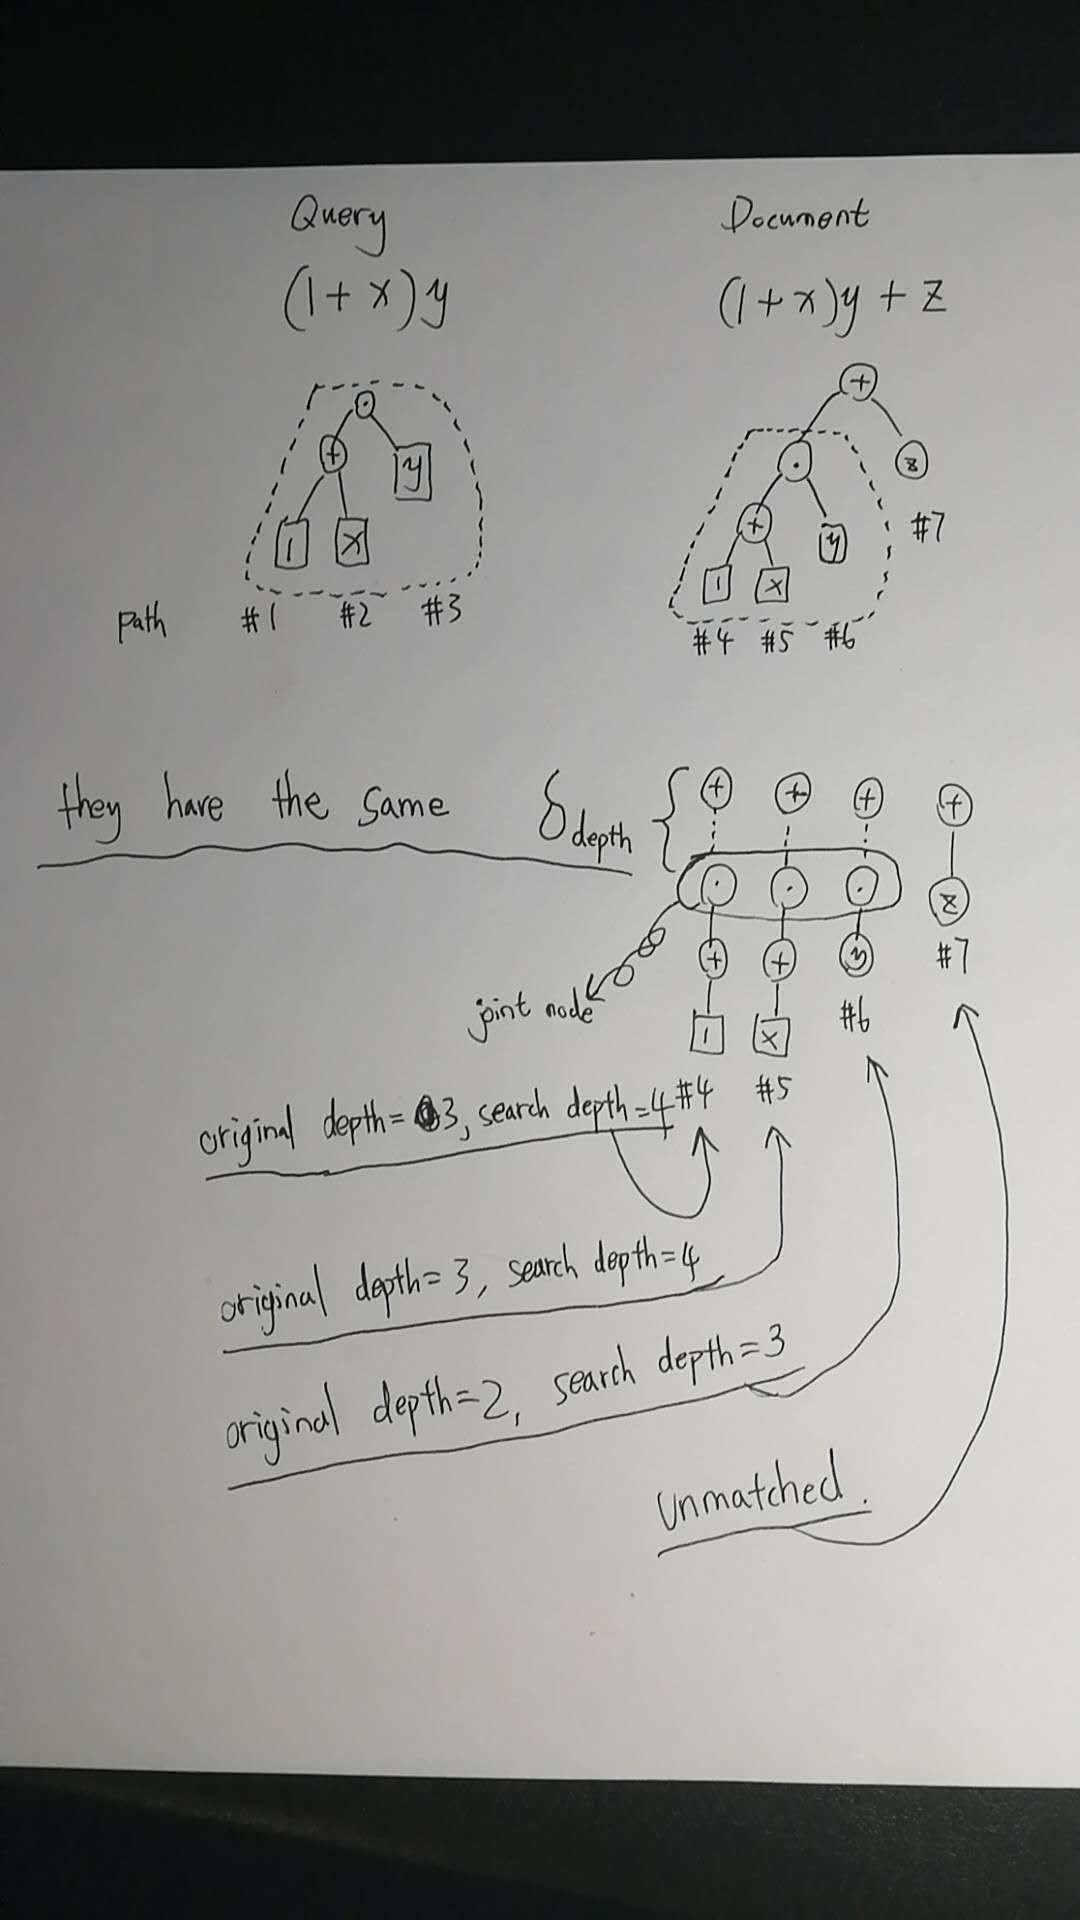
\includegraphics[width=0.5\textwidth]{easyforu.jpg}
\caption{\label{fig:frog}Example of matching depth and $\delta_\text{depth}$}
\end{figure}

\subsection{Possible scoring functions (iii.)}
\textbf{Explanation on the scoring formula: Matched path scores / depth-from-root + missing\_paths + 1.0}

The proposed formula for ranking is borrowed from original mark-and-cross scoring schema, since all the original mark-and-cross algorithm want to know (the input) is the hitlist information, and since we can get the hitlist for particular matching subtree after the end of prefix-path alignment algorithm, we can consider to apply mark-and-cross scoring into each of the subtrees without interfering with each other (if we just apply it to the entire expression hitlist, there might be conflict between resulting embedding from prefix-alignment and symbol set alignment). The proposed scoring formula is actually:
$$
\begin{aligned}
\text{score}
&= \dfrac {\text{symbol set similarity}} {\delta_{\text{depth}} + \delta_{\text{breath}} + 1} \\
&= \dfrac {\text{symbol set similarity}} {|\text{query original depth} - \text{search depth}| + |\text{query original number of paths} - \text{number of paths matched}| + 1}
\end{aligned}
$$
And yes, the one here is a constant, it is just a math trick to prevent dividing-by-zero.

\subsection{Possible scoring functions (iii. 1)}
\textbf{What is the motivation for using a fraction here?}

The fraction here is trying to penalize the structure matching "portion/percentage", so even if the query subexpression is perfectly embedded into its document expression in terms of both symbol set and structure, if the subexpresion is too "small" compared to its embedded document expression structure, then the score should penalize this case. And by "small" I intuitively choose to use the breath delta (difference in terms of number of paths) and height delta (difference in terms of matching depth) to represent the "percentage" of document expression being matched.

\subsection{Possible scoring functions (iii. 2)}
\textbf{The depth from root and path lengths don't seem to be represented uniformly in this metric}

So the proposed formula only cares the delta of depth (and delta of breath), please see figure~\ref{fig:frog}, although each path is of different depth, they all have the identical delta depth. This is because starting from the root it gets embedded, if a node from path A is embedded, then the same node from different path B in the same tree is also embedded because they are the same node (joint node), so they all have the same delta depth value which corresponds to the number of nodes beyond root that (all of them) get embedded into document tree.

\subsection{Possible scoring functions (iii. 3)}
\textbf{Why do we score number of paths, but not number of symbols matched in these paths?}
Sorry for this confusion, the score-by-path is actually borrowed from original Approach0 formula, since we are using prefix-path now and it has its own scoring schema (by number of matched paths also), it is arguably "repeated" to consider path number in final scoring schema again where both symbol set similarity and structure similarity is evaluated. You can forget about the final formula that combines everything, the more general way to define our overall scoring is just: We have a score $S_p$ (tuple) for prefix-path structure similarity, and we also have a score $S_s$ for symbol set similarity, and we will use some function (yet to be determined in near future) to combine or add other parameters (such as matching depth) into the overall scoring function $f(S_p, S_s)$. I shouldn't determine the final $f$ function this early.

\section{Comment on initial results from prefix-path matching}
Current evaluation has been done on prefix-path based method without symbol set similarity awareness, so the real power of this method is not shown and current metrics has already demonstrated a good potential in terms of precision metrics.
Please see Table~\ref{tab:frog} for the summary of \verb|trec_eval| (full relevance) results from different systems.

\begin{table}
\begin{center}
\begin{tabular}{lllr}
\hline
\multicolumn{3}{c}{Evaluation results} \\
\cline{1-3}
Prefix-path based & Original A0 & Tangent@NTCIR-12 (run4) & Metrics \\
\hline
0.3200            & 0.3556      & 0.5300   & Precision@5    \\
0.3333            & 0.2556      & 0.3700   & Precision@10    \\
0.2222            & 0.1704      & 0.3167   & Precision@15   \\
0.1667            & 0.1278      & 0.2775   & Precision@20    \\
0.1111            & 0.0852      & -        & Precision@30   \\
0.0333            & 0.0256      & -        & Precision@100   \\
0.0167            & 0.0128      & -        & Precision@200   \\
0.0067            & 0.0051      & -        & Precision@500   \\
0.0033            & 0.0026      & -        & Precision@1000  \\
0.1063            & 0.3275      & 0.5530(comb), 0.4207(core-SLT), 0.4241(core-OPT) & bpref   \\
\hline
\end{tabular}
\caption{\label{tab:frog}Preliminary results comparison (full relevance) \cite{Davila2016Tangent3AT, DavilaSigir}}
\end{center}
\end{table}

As you can see, prefix-path based method has surpassed original Approach0 in every matrices except for Precision@5 which is expected since original Approach0 is very strict in structure. Prefix-path based method offer great fuzziness so that many results which cannot return in original Appraoch0 are searchable now, and it also performs very well in all other precision metrics but fails to perform well for bpref mainly because it does not support symbol set matching currently, so the ranking order will have less advantage even having higher precision.

\bibliographystyle{alpha}
\bibliography{sample}

\end{document}
